\documentclass{article}
\usepackage[utf8]{inputenc}
\usepackage{csquotes}
\usepackage[catalan]{babel}
\usepackage{amssymb} %Para usar símbolos matemáticos
%\usepackage{amsmath} %Para usar entornos matemáticos
\usepackage{float}
\usepackage{amsmath}


%Composición
\usepackage[a4paper,
%showframe,
    %total={450pt, 630pt},
    left=80pt,
    right=80pt,
    top=80pt,
    bottom=80pt,   
    headsep=10pt]{geometry}
\usepackage{setspace}
\renewcommand{\baselinestretch}{1.4}
\parskip=4pt
%\setlength\parindent{0pt} %Quitar sangría al principio de párrafo



%Paquet per afegir codi maco
\usepackage{caption}
\DeclareCaptionFont{orange}{\color{orange}}
\captionsetup{labelfont=orange} 

\usepackage[usenames,dvipsnames,table,xcdraw]{xcolor}
\usepackage{listings}
\lstdefinestyle{sql}{
        basicstyle=\ttfamily,
        keywordstyle=\color{red},
        stringstyle=\color{Mahogany},
        commentstyle=\color{PineGreen},
        breaklines=true,
        showstringspaces=false,
        numbers=left,
        backgroundcolor=\color{gray!20},
        numberstyle=\tiny\color{gray},
        stepnumber=1,
        numbersep=10pt}
\lstset{language=R,
        basicstyle=\ttfamily,
        keywordstyle=\color{blue},
        stringstyle=\color{Mahogany},
        commentstyle=\color{PineGreen},
        breaklines=true,
        showstringspaces=false,
        numbers=left,
        backgroundcolor=\color{gray!20},
        numberstyle=\tiny\color{gray},
        stepnumber=1,
        numbersep=10pt}
        \usepackage[usenames,dvipsnames]{xcolor}

%Citas y referencias
\usepackage{hyperref}
\hypersetup{urlcolor=cyan}

\usepackage[style=numeric]{biblatex}
\addbibresource{references.bib}

%comentaris multilinea
\usepackage{comment}

%Imágenes
\usepackage{graphicx}
\graphicspath{ {./} }
\usepackage[justification=centering]{caption}

%Cabeceras
\usepackage{fancyhdr}
\fancypagestyle{logos}
{
    \fancyhf{}
    \fancyhead[L]{
\includegraphics[scale=0.04]{Images/upc.png}}    
    \fancyhead[R]{
\includegraphics[scale=0.04]{Images/fib.png}}
}

%Inicio del documento
\begin{document}

\begin{titlepage}
\thispagestyle{logos}
\vspace*{1.5cm}
\centering
{\bfseries\LARGE Universitat Politècnica de Catalunya \par}
\vspace{1cm}
{\scshape\Large Facultat d'Informàtica de Barcelona \par}
\vspace{2.5cm}
{\scshape\Huge Anàlisi i modelatge dels top 40 cançons setmanals de Spotify\par}
\vspace{0.5cm}
{\scshape\LARGE Entrega del D3 \par}
\vspace{2.5cm}
{\itshape\Large Grau en Intel·ligència Artificial \par}
{\itshape\Large Preprocessament i Models Avançats d'Anàlisi de Dades\par}
\vfill
{\Large Autors: \par}
{\Large \textbf{Roger Baiges, Pablo Barrenechea, Anna Casanovas, Pau Hidalgo, Abril Risso, Cai Selvas.}  \par}
\vfill
{\Large \today \par}
\end{titlepage}


\newpage
\tableofcontents


\newpage
\section{Secció 1}

Esta es la primera sección del documento, aquí se montará la portada y el índice.

Así se debería citar una imagen: figura \ref{fig:Section1_Imagen1}

\begin{figure}[H]
    \centering
    
\includegraphics[width=0.4\textwidth]{Images/Section1/Imagen1.jpg}
    \caption{Imatge de la duració mitjana per mesos al llarg del temps}
    \label{fig:Section1_Imagen1}
\end{figure}

Y así se podría construir un conjunto de dos imágenes, una al lado de otra (ver figuras \ref{fig:Section1_dobleImagen1} y \ref{fig:Section1_dobleImagen2}).

\begin{figure}[H]
\centering
    \begin{minipage}{.4\textwidth}
        \centering
        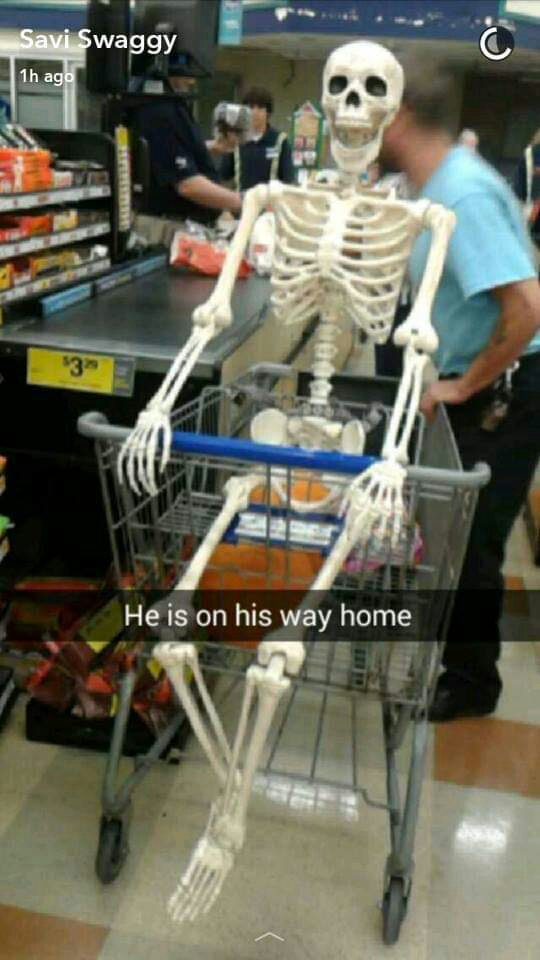
\includegraphics[width=0.95\linewidth]{Images/Section1/doble_imagen1.jpg}
        \caption{Mi colega \\ así se introducen \\ saltos de línea en \\ la caption}
        \label{fig:Section1_dobleImagen1}
    \end{minipage}%
    \begin{minipage}{.4\textwidth}
        \centering
        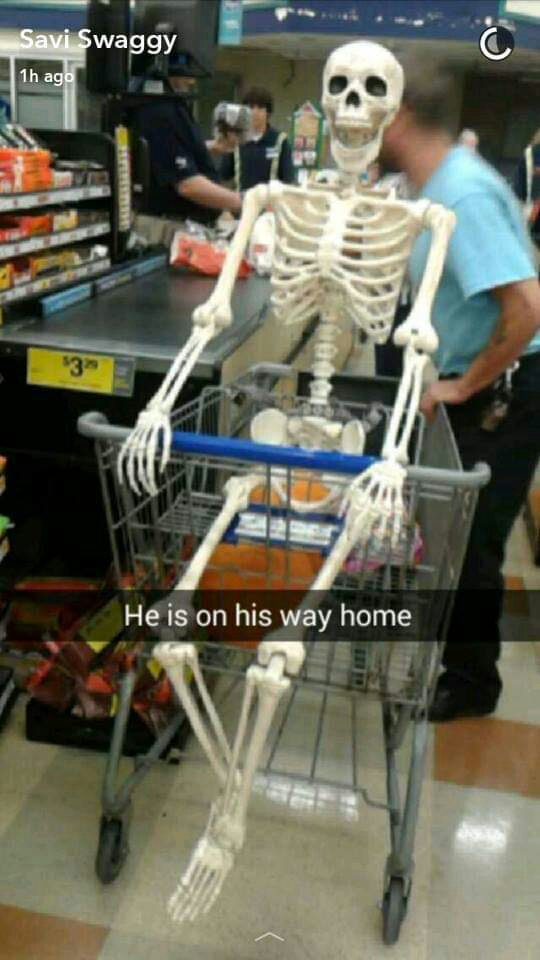
\includegraphics[width=0.95\linewidth]{Images/Section1/doble_imagen2.jpg}
        \caption{Otro esqueleto (por favor, fuera coñas, pongan caption}
        \label{fig:Section1_dobleImagen2}
    \end{minipage}%
\end{figure}

\subsection{Subsecció 2: Taula}

Hay muchas maneras de hacer una tabla, cada uno que escoja su favorita, pero por favor, referenciar también las tablas, como la tabla \ref{tab:Section1_tabla}

\begin{table}[H]
\centering
\begin{tabular}{
|>{\columncolor[HTML]{C0C0C0}}c |c|c|c|c|c|c|}
\hline
{\color[HTML]{000000} \textit{\textbf{k}}} & 2      & 3       & 4       & 5      & 6       & 7       \\ \hline
\textit{\textbf{mean}}                     & 0.2120 & 0.16028 & 0.16204 & 0.1327 & 0.13063 & 0.13494 \\ \hline
\end{tabular}
\caption{Valors de silhouette}
\label{tab:Section1_tabla}
\end{table}



\end{document}